% !TeX encoding = UTF-8
% !TeX program = xelatex
\documentclass[12pt, a4paper]{article}
\usepackage{xeCJK} % 须放在\usepackage{}列中足够前的位置
\usepackage{fontspec}
\usepackage{graphicx}
\usepackage{caption}
\usepackage{enumerate}
\usepackage{setspace}
\usepackage{array} % 製作表格必須的宏包
\usepackage{tabularx} % 自動調整列寬的表格宏包
\usepackage{adjustbox}
\setCJKfamilyfont{heiti}{Heiti TC}
\CJKfamily{heiti}
\setmainfont{Arial}
\setstretch{1.5}


\begin{document}
\begin{center}
  {\Huge 邏輯設計實驗} \\[2.5cm]
  {\Huge Lab10} \\[1.5cm]
  {\Huge 閂鎖器與正反器} \\ [4.5cm]
  \hspace{.6in}
  \begin{minipage}[t]{.4\linewidth}
    {\Large 班級:資訊一甲}\\[0.5cm]
    {\Large 學號:D1109023}\\[0.5cm]
    {\Large 姓名:楊孟憲}
  \end{minipage}    
\end{center}

\newpage
%\fontsize{30pt}{36pt}\selectfont 
%\normalsize

\begin{description}
  \fontsize{22pt}{25pt}\selectfont 
    \item [一、]摘要 
      \begin{enumerate}
        \fontsize{20pt}{22pt}\selectfont
          \item 組合邏輯與續向邏輯 
            \begin{description}
              \fontsize{16pt}{20}\selectfont
                \item [$\bullet$] 邏輯電路分為「組合邏輯」與「序向邏輯」兩類。
                \item [$\bullet$] 組合邏輯的輸出是「現在輸入」的函數,也就是說,有相同的輸入必然有相同的輸出。
                \item [$\bullet$] 序向邏輯中的輸出不僅是「現在輸入」的函數,同時也是「目前狀態」的函數;換言之,系統中必須擁有能將這些狀態記憶住的裝置,這就是閂鎖器/正反器的功能。\\
              \normalsize
            \end{description}
            \item 閂鎖器 
              \begin{description}
                \fontsize{16pt}{20}\selectfont
                  \item [$\bullet$] S  :資料設定(Data Set)
                  \item [$\bullet$] R  :資料重置(Data Reset)
                  \item [$\bullet$] 邏輯符號 \\[.5cm]
                  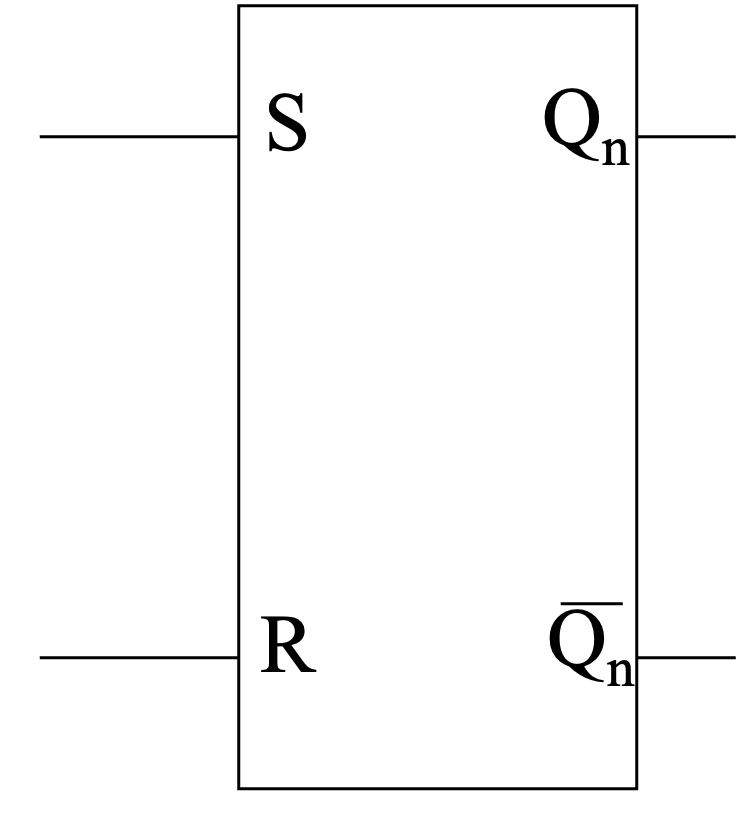
\includegraphics[width=5cm]{./image/latch.png} \\
                  \item[$\bullet$] 真值表 \\[.5cm]
                  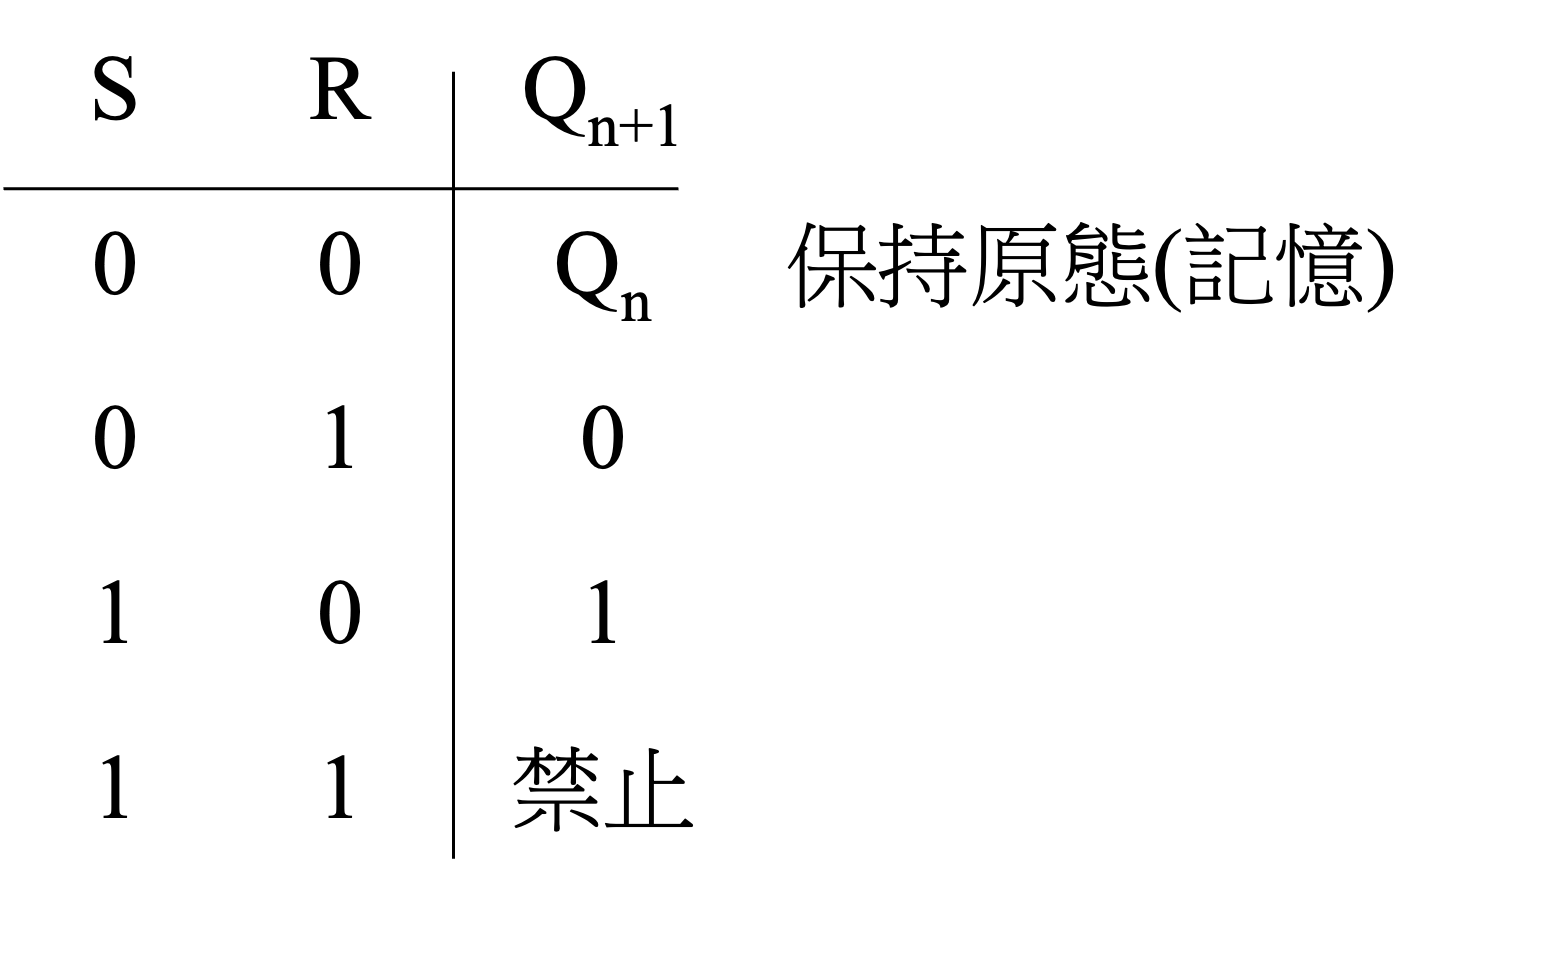
\includegraphics[width=10cm]{./image/latch_truthtable.png}
                  \item[$\bullet$] 電路圖 \\[.5cm]
                  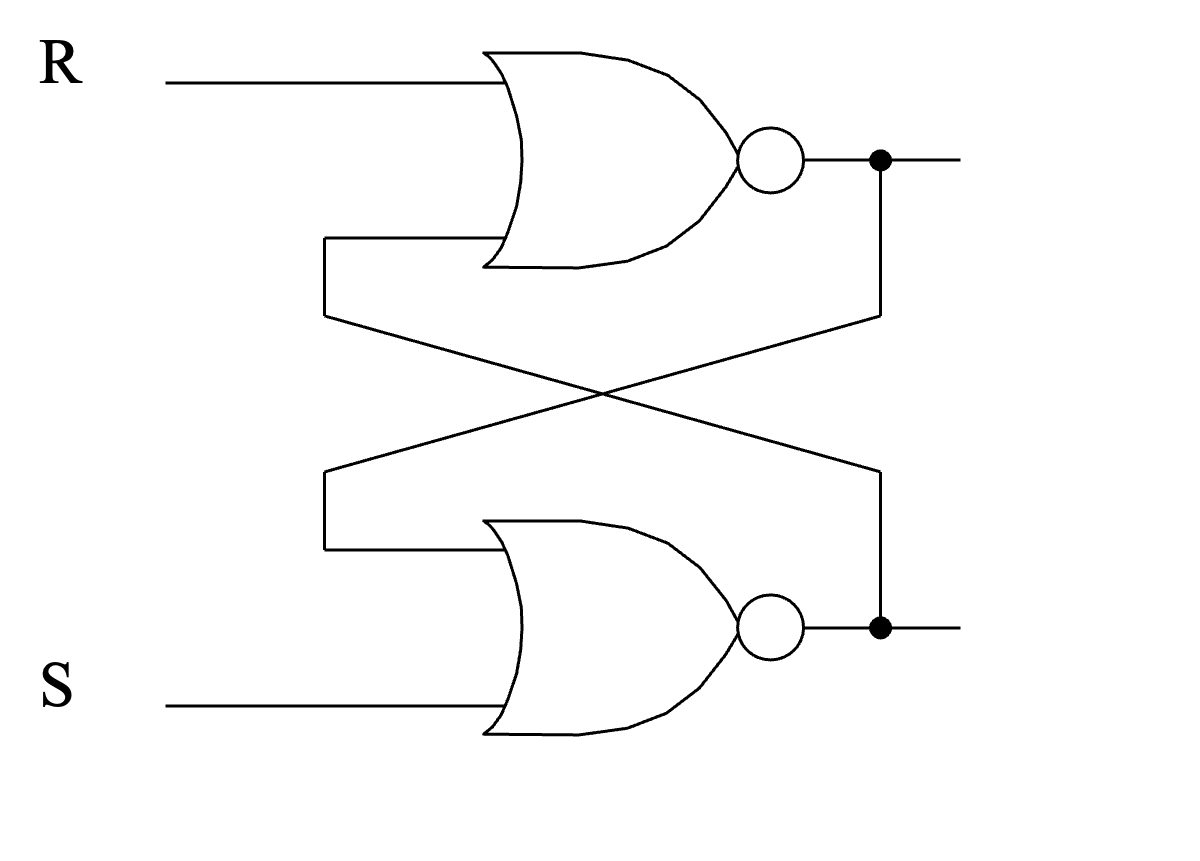
\includegraphics[width=8cm]{./image/Latch_logic.png}
                \normalsize
              \end{description}

              \item 正反器(Filp-Flop) \\
              \begin{description}
                \fontsize{16pt}{20}\selectfont
                  \item [(1)] 時脈訊號可用來控制正反器輸出狀態之轉變,可藉由時脈訊號之改變瞬間,對正反器輸入訊號取樣後,以決定正反器之輸出狀態而這改變瞬間稱為正反器的觸發。

                  \item [(2)] 在數位系統中,邊緣觸發方式有兩種:\\
                  (a) 正緣觸發(0→1)\\
                  (b) 負緣觸發(1→0)\\
                  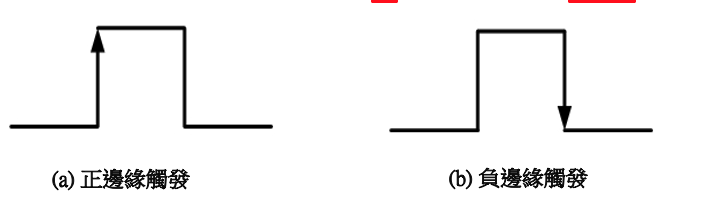
\includegraphics[width=10cm]{./image/filp-flop.png}

                  \item[(3)] 閂鎖器與正反器相異處:\\
                  閂鎖器:不需時脈信號觸發即可做狀態的改變\\
                  正反器:需配合時脈信號觸發才可做狀態改變\\
                  
                \normalsize  
              \end{description}
            
              \item 實驗 
              \begin{description}
                \fontsize{16pt}{20}\selectfont
                  \item [(1)] D型 閂鎖器 (D Latch) 
                  \item [(2)] D型 正反器 (D Flip-Flop) 
                  \item [(3)] An 8-bit Register with asynchronous reset \\
                \normalsize  
              \end{description}

        \normalsize
      \end{enumerate}
    \item [二、]實驗結果
      \begin{description}
        \fontsize{20pt}{22pt}\selectfont
        \item 實驗一 (D型 閂鎖器 (D Latch))
          \fontsize{16pt}{18pt}\selectfont
            \begin{description}
              \item [$\bullet$]實作一個 D型 閂鎖器
              \item [$\bullet$]Use SW0 as the clock\\
              \fontsize{18pt}{20pt}
                \item [(1)]電路圖 \\[.3cm]
                  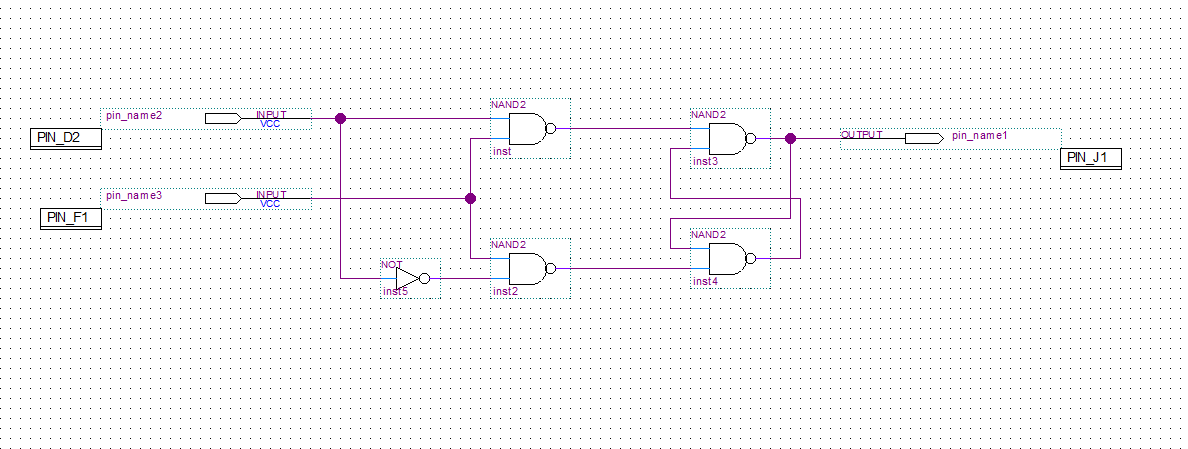
\includegraphics[width=13cm]{./image/ex1.PNG}
                \item [(2)] 波形圖 \\[.3cm]
                  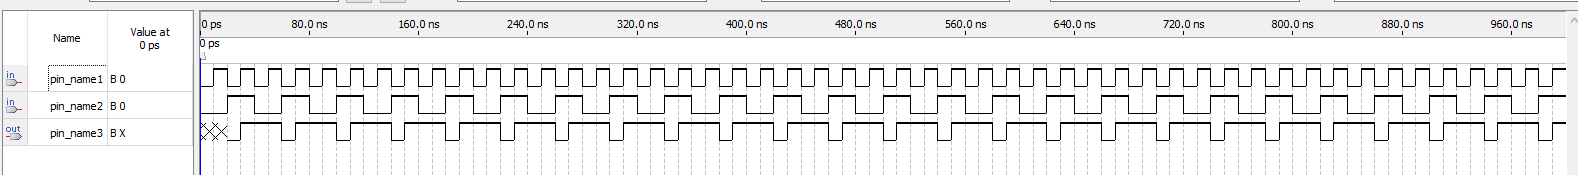
\includegraphics[width=13cm]{./image/EX1_1.PNG}  \\          
            \end{description}
          \normalsize
          
          \fontsize{20pt}{22pt}\selectfont
          \item 實驗二 (D型 正反器 (D Flip-Flop))
          \fontsize{16pt}{18pt}\selectfont
            \begin{description}
              \item [$\bullet$] 實作一個 主僕式 D型 正反器
              \item [$\bullet$] Use Button2 as the clock \\
              \fontsize{18pt}{20pt}
                \item [(1)]電路圖 \\[.3cm]
                  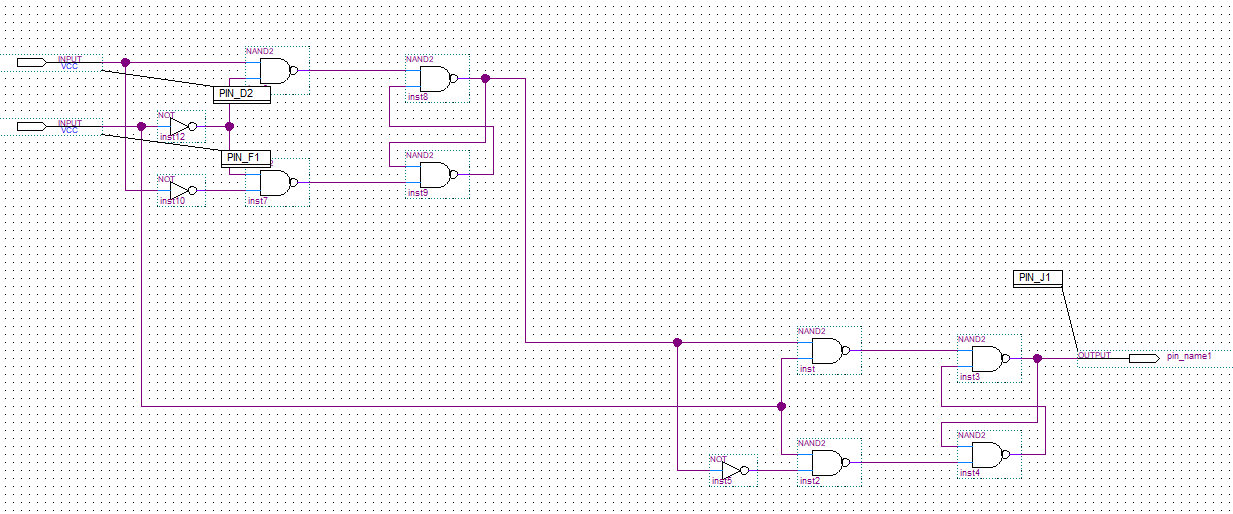
\includegraphics[width=13cm]{./image/ex2.PNG}
                \item [(2)] 波形圖 \\[.3cm]
                  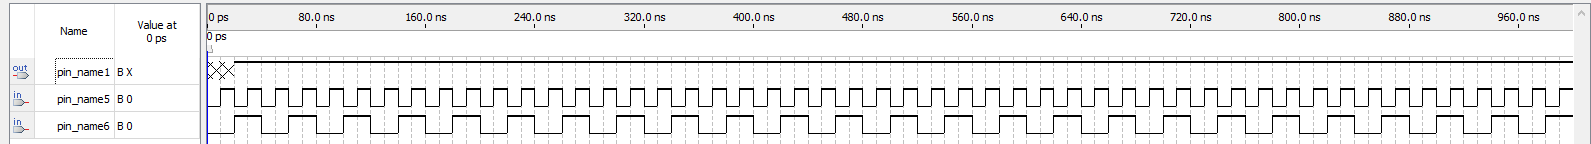
\includegraphics[width=13cm]{./image/EX2_2.PNG} \\             
            \end{description}
          \normalsize


          \fontsize{20pt}{22pt}\selectfont
          \item 實驗三 (An 8-bit Register with asynchronous reset)
          \fontsize{16pt}{18pt}\selectfont
            \begin{description}
              \item [$\bullet$]請使用八個具非同步 reset 的 D 正反器 (函式庫提供), 實作一個具非同步 reset 的八位元暫存器 (D7~D0為兩個BCD數字)
              \item [$\bullet$]使用兩個七段顯示器, 顯示暫存器的內容
              \item [$\bullet$]Use Button0 as an active-low asynchronous reset
              \item [$\bullet$]Use Button2 as the clock\\
              \fontsize{18pt}{20pt}
                \item [(1)]電路圖 \\[.3cm]
                  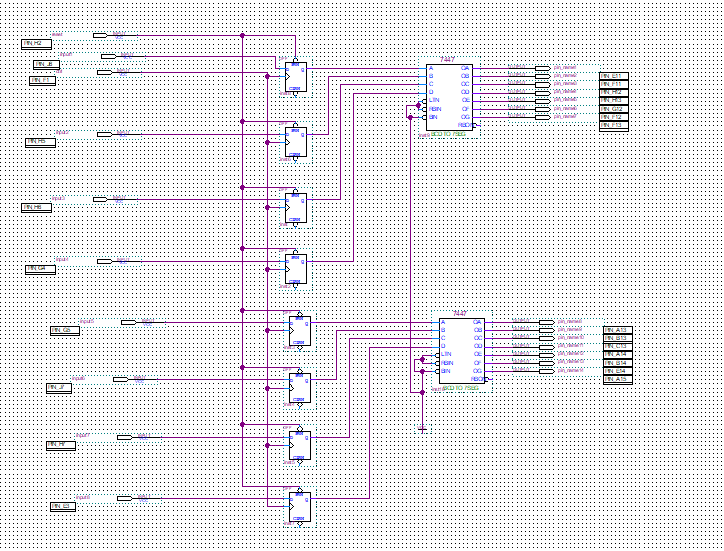
\includegraphics[width=13cm]{./image/ex3.PNG}\\         
            \end{description}
          \normalsize

        \normalsize
      \end{description}
    \item [三、]問題討論心得 \\[.6cm]
      \begin{minipage}[t]{\linewidth}
        \fontsize{16}{18}\selectfont
          這次的實驗讓我學習到如何實作一個主僕式D型正反器等等,透過設計電路並進行模擬,成功地實現了正反器的功能。在這個過程中,我深刻體驗到了電路設計的重要性,每一個元件都必須精確地配置,才能確保整個電路的正確運作。此外,我也學到了如何使用電路模擬軟體進行測試和驗證,以確認電路的穩定性和可靠性。這次的實驗讓我更深入地理解了數位電路的運作原理和設計方法,對我的未來學習和研究有著極大的幫助。
        \normalsize  
      \end{minipage}
  \normalsize
\end{description}

\end{document}


